\scanpage{41}

donnée des commutativités $\alpha_{D^*U}$, et écrire les conditions de compatibilité avec $\alpha,\alpha'$ et $k,k'$. La donnée de $\alpha_{D^*,U}$ équivaut à celle de systèmes d'éléments
\[
\boxed{\beta_{i'}\in\mathcal E'}\qquad(i'\in I')
\]
\deleted{\illegible{1}}\inserted{tels que} l'on ait, dans les diagrammes
\diagram{\begin{tikzcd}[ampersand replacement=\&]
G'_{i'} \arrow[r,"\rho'_{i'}"] \arrow[d,"f_{i'}"'] \& \mathcal E' \arrow[d,"f_{\mathcal E}"] \\
G_{\tau i'} \arrow[r,"\rho_{\tau i'}"'] \& \mathcal E
\end{tikzcd}}
la relation
\[
f_{\mathcal E}\rho'_{i'}=\operatorname{int}(\beta_{i'})\rho_{\tau i'}\circ f_{i'}.
\]

Reste à exprimer les \inserted{deux} compatibilités \deleted{avec} de
$(\unsure{f_{D^*}},f_D,f_U,\unsure{\alpha_{D^*D}},\alpha_{De},\alpha_{D^*U},\alpha_{Ue})$ avec
lui-= et avec $K$ --- la deuxième compatibilité est simplement la compatibilité des $f_{i'}$ avec les $k'_{i'},k_i$, i.e.
\[
f_{i'}\circ k'_{i'}=k_i\qquad(i=\tau i')
\]
et la première \uline{sauf erreur} s'exprime par la ``commutativité''
\[
\deleted{\unsure{\rho(\beta_{i'})|p(\beta_{i'})}}\alpha\gamma'_{i'}
 =\inserted{\unsure{\rho(\beta_{i'})|p(\beta_{i'})}}\gamma_i\alpha_{i'}
 \qquad\forall i'\in I'
\]
\[
\boxed{\alpha_{i'}=\gamma_i^{-1}\unsure{\rho|p}(\beta_{i'}^{-1})\alpha\gamma'_{i'}}
\]
\margin{40}

\scanpage{42}
\mspage{19}

En résumé, les \unsure{homs}, dans un \inserted{syst. de} \deleted{\illegible{1}} diagrammes comm.
\diagram{\begin{tikzcd}[ampersand replacement=\&, column sep=small]
1 \arrow[r] \& T(\bar K) \arrow[r,"k_i"] \arrow[dr] \& \mathcal E_i \arrow[r,"p_i"] \arrow[dr,"\rho_i"] \& \Gamma \arrow[dr,"\operatorname{int}(\gamma_i)"] \& \\
\& 1 \arrow[r] \& \pi \arrow[r] \& \mathcal E \arrow[r,"p"'] \& \Gamma
\end{tikzcd}\qquad$(i\in I)$}
d'un système analogue, relatif à un ens. d'indices $I'$, est donné par une application
\[
\tau:I'\longrightarrow I
\]
et pour tout $i'\in I'$, posant $i=\tau(i')$, d'un système de flèches verticales $f_{i'}\inserted{{}:\mathcal E'_{i'}\longrightarrow\mathcal E_i}$, et d'une flèche \inserted{verticale} $f_{\mathcal E}:\mathcal E'\longrightarrow\mathcal E$, enfin \deleted{de systèmes} \deleted{$\alpha\in\Gamma$ et} d'un système d'éléments $\beta_{i'}\in\mathcal E$ et d'un $\alpha\in\Gamma$, \deleted{satisfaisant} s'insérant dans le syst. de diagrammes
\diagram{\begin{tikzcd}[ampersand replacement=\&,column sep=1.3em,row sep=2.2em]
1\arrow[rr] \& \& T(\bar K)\arrow[rr,"k'_{i'}"]\arrow[dr,"\varepsilon'_{i'}"']\arrow[dd,"d_{i'}"'] \& \& \mathcal E'_{i'}\arrow[rr,"p'_{i'}"]\arrow[dr,hook,"\rho'_{i'}"]\arrow[dd,"f_{i'}"' near start] \& \& \Gamma\arrow[dr,"\operatorname{int}(\gamma'_{i'})"]\arrow[dd,"\operatorname{int}(\alpha_{i'})"' near start] \& \\
\& 1\arrow[rr] \& \& \pi'\arrow[rr]\arrow[dd] \& \& \mathcal E'\arrow[rr,"p'"]\arrow[dd,"f_{\mathcal E}" near start] \& \& \Gamma\arrow[dd,"\operatorname{int}(\alpha)"] \\
1\arrow[rr] \& \& T(\bar K)\arrow[rr,"k_i"]\arrow[dr,"\varepsilon_i"'] \& \& \mathcal E_i\arrow[rr,"p_i"]\arrow[dr,hook,"\rho_i"'] \& \& \Gamma\arrow[dr,"\operatorname{int}(\gamma_i)"] \& \\
\& 1\arrow[rr] \& \& \pi\arrow[rr] \& \& \mathcal E\arrow[rr,"p"'] \& \& \Gamma
\end{tikzcd}
[Prisme : les deuxième et quatrième lignes sont décalées vers la droite. La flèche verticale $d_{i'}$ entre les deux $T(\bar K)$ est tracée d'un trait doublé ; $\pi'\longrightarrow\pi$ sans étiquette. Sous la flèche $p_i$, près de la pointe de $\rho_i$, $\unsure{\beta_{i'}}$ surchargé ; plus loin sur la même flèche, près de la pointe vers $\Gamma$, un signe surchargé \illegible{1}.]}

\margin{\uline{NB} Comme les $\mathcal E_i\hookrightarrow\mathcal E$ sont injectifs, \deleted{le} $f_{i'}$ est connu quand on connait $f_{\mathcal E}$ et $\beta_{i'}$ (l'existence \unsure{de|des} $f_{i'}$ est donc une condition sur les couples $f_{\mathcal E},\beta_{i'}$ \illegible{1} \unsure{savoir} que $\operatorname{int}(\beta_{i'})^{-1}f_{\mathcal E}\rho'_{i'}$ \unsure{$\mathcal E'_{i'}$} dans $\unsure{\rho_i(\mathcal E_i)|p_i(\mathcal E_i)}$)}

\margin{\uline{NB.} OPS les $\gamma'_{i'},\gamma_i$ égaux à $1$ (en choisissant l'image de $\unsure{\psi|\varphi}\sigma(D_i^*)$ \unsure{sur} $\operatorname{Spec}(\bar K)$ via l'isom. de $\varphi(\rho(D_i^*))\simeq\varphi(\unsure{\widetilde U|\widetilde U_i})$ \unsure{avec} $\operatorname{Spec}\bar K$}

\unsure{où on a} posé
\[
(*)\quad\alpha_{i'}=\gamma_i^{-1}p(\beta_{i'}^{-1})\alpha\gamma'_{i'}
\qquad\text{i.e.}\quad\deleted{\illegible{1}}\ \alpha\gamma'_{i'}=p(\beta_{i'})\gamma_i\alpha_{i'}
\]
et \unsure{i.e.|où} la face \inserted{verticale} postérieure des prismes est commutative (deux conditions, sur deux carrés), la face \inserted{verticale} antérieure aussi (c'est \uline{une} condition, sur le carré de droite, l'autre carré
\margin{41}

\scanpage{43}

comm. s'en déduit par définition de $\pi'\longrightarrow\pi$ comme induit par $f_{\mathcal E}\ldots$), la face verticale gauche du cube de droite étant commutative modulo l'isom. de commutativité $\operatorname{int}(\beta_{i'})$, et la face verticale droite étant \deleted{\unsure{cont}}commutative (non seulement, par la condition précédente, sur
\[
\unsure{\Gamma'_{i'}}=\operatorname{Im}(\mathcal E'_{i'}\xrightarrow{p'_{i'}}\Gamma),
\]
mais sur $\Gamma$ tout entier) en vertu de la relation plus précise $(*)$.

\figure{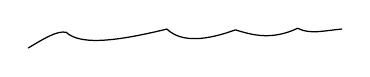
\begin{tikzpicture}[x=1cm,y=1cm,line cap=round,line join=round]
\draw[line width=0.45pt] (0,0) .. controls (0.20,0.12) and (0.36,0.22) .. (0.48,0.20)
.. controls (0.67,0.02) and (1.18,0.10) .. (1.76,0.24)
.. controls (1.95,0.06) and (2.27,0.10) .. (2.63,0.23)
.. controls (2.83,0.17) and (3.08,0.09) .. (3.42,0.25)
.. controls (3.58,0.17) and (3.75,0.22) .. (3.98,0.24);
\end{tikzpicture}}

Catégorie bordélique précisée (correspondant à un $\Pi_U$ \uline{connexe}) :

Ces objets sont les \deleted{couples $(I$, \unsure{systèmes}}\inserted{homs de gr.} profinis \deleted{(\unsure{indexés} par un ens. fini $I$) de l'hom}
\[
\mathcal E\xrightarrow{p}\Gamma
\]
(donnant naissance à une suite exacte :
\[
1\longrightarrow\pi\xrightarrow{\unsure{k|\kappa}}\mathcal E\xrightarrow{p}\Gamma
\]
)
et un ens. \inserted{fini} de sous-groupes (indexé par un ens $I$ d'indices)
\[
\mathcal E_i\overset{\rho_i}{\lhook\joinrel\longrightarrow}\mathcal E,
\]
et d'isomorphismes
\[
\mathcal E_i\cap\pi\overset{k_i}{\simeq}T(\bar K)
\]
\margin{42}

\scanpage{44}
\mspage{20}

Un hom d'un système
$(\mathcal E',p',(\mathcal E'_{i'})_{i'\in I'},(k'_{i'})_{i'\in I'})$
dans un syst.
$(\mathcal E,p,(\mathcal E_i)_{i\in I},(k_i)_{i\in I})$
est donné par par un hom
\[
f:\mathcal E'\longrightarrow\mathcal E
\]
\[
\beta_{i'}\in\mathcal E\quad(i'\in I'),\qquad\alpha\in\Gamma,
\]
tels que l'on ait les conditions :

\figure{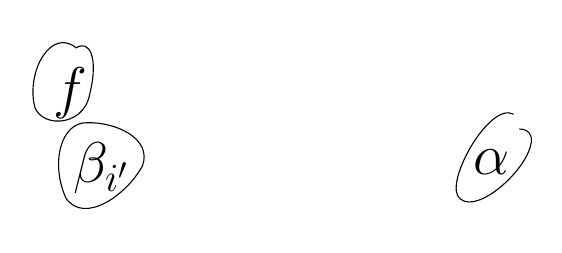
\begin{tikzpicture}[x=1cm,y=1cm,line cap=round,line join=round]
\begin{scope}[yshift=-0.35cm]
\node[font=\fontsize{22}{24}\selectfont] at (0,1.30) {$f$};
\draw (0.08,1.88) .. controls (-0.22,2.13) and (-0.53,1.64) .. (-0.46,1.19)
.. controls (-0.43,0.86) and (0.17,0.85) .. (0.25,1.29)
.. controls (0.37,1.77) and (0.24,1.99) .. (0.08,1.88);
\end{scope}
\node[font=\fontsize{22}{24}\selectfont] at (0.40,0) {$\beta_{i'}$};
\draw (0.22,0.58) .. controls (-0.12,0.59) and (-0.25,0.06) .. (-0.05,-0.38)
.. controls (0.18,-0.71) and (0.71,-0.35) .. (0.92,0.03)
.. controls (1.05,0.38) and (0.58,0.59) .. (0.22,0.58);
\node[font=\fontsize{22}{24}\selectfont] at (5.35,0.08) {$\alpha$};
\draw (5.63,0.69) .. controls (5.32,0.85) and (4.72,-0.23) .. (4.96,-0.39)
.. controls (5.18,-0.57) and (5.77,-0.05) .. (5.85,0.29)
.. controls (5.89,0.42) and (5.82,0.50) .. (5.71,0.50);
\end{tikzpicture}}

\margin{Les $\beta_{i'}$ pas uniques (si $\beta_{i'}$ convient, aussi $\gamma\beta_{i'}$, avec $\unsure{\gamma|\gamma_i}\in\operatorname{Im}k_i$). Mais $\alpha$ unique \unsure{?!|??}}

$1^\circ)$\quad $p\circ f_{\mathcal E}=\operatorname{int}(\alpha)\,p'$

$2^\circ)$\quad $\forall i'\in I',\quad\exists i\in I$ (unique!) tel que
\[
\operatorname{int}(\beta_{i'}^{-1})f(\mathcal E'_{i'})\subset\mathcal E_i
\]
et un entier $d_{i'}\in\mathbb N^*$ tel que
\[
\operatorname{int}(\beta_{i'}^{-1})f\,k'_{i'}
 =k_i\circ(d_{i'}\cdot\operatorname{id}_{T(\bar K)})
\]

\margin{NB : $d_{i'}$ est aussi unique\ldots}

\margin{[donc $\operatorname{int}(\beta_{i'}^{-1})\overbrace{\unsure{\operatorname{Im}(fk'_{i'})|\operatorname{Im}k'_{i'}}}^{L'_{i'}}\subset\underbrace{\operatorname{Im}k_i}_{L_i}$ et \unsure{même} \deleted{\unsure{cette} image} $\operatorname{int}(\beta_{i'}^{-1})\unsure{L'_{i'}}=d_{i'}L_i$.]}

\figure{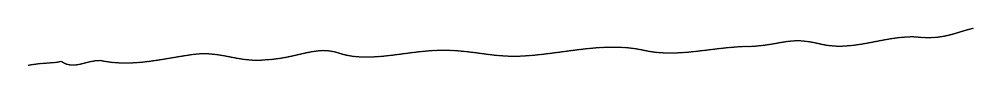
\begin{tikzpicture}[x=1cm,y=1cm,line cap=round,line join=round]
\draw[line width=0.45pt] (0,0) .. controls (0.22,0.04) and (0.30,0.02) .. (0.42,0.05)
.. controls (0.58,-0.07) and (0.73,0.07) .. (0.92,0.06)
.. controls (1.30,-0.02) and (1.64,0.07) .. (2.04,0.13)
.. controls (2.44,0.20) and (2.64,0.03) .. (3.02,0.07)
.. controls (3.43,0.09) and (3.66,0.26) .. (3.96,0.15)
.. controls (4.37,0.02) and (4.86,0.21) .. (5.35,0.19)
.. controls (5.79,0.17) and (5.95,0.08) .. (6.44,0.13)
.. controls (6.94,0.18) and (7.37,0.29) .. (7.82,0.19)
.. controls (8.26,0.09) and (8.70,0.24) .. (9.18,0.24)
.. controls (9.58,0.26) and (9.66,0.37) .. (10.06,0.27)
.. controls (10.48,0.17) and (10.87,0.38) .. (11.28,0.36)
.. controls (11.62,0.32) and (11.78,0.42) .. (12.00,0.47);
\end{tikzpicture}}

Je m'aperçois qu'il vaut mieux remplacer les $\beta_{i'}$ par les $\beta_{i'}^{-1}$, i.e. prendre l'iso. de commutation plutôt dans le sens
\[
f_{\mathcal E}\rho'_{i'}\xrightarrow{\beta_{i'}}\rho_i f_{i'}
\]
qu'en sens inverse. De plus, conceptuellement le diagramme
\diagram{\begin{tikzcd}[ampersand replacement=\&]
\& \Pi_{D^*}\arrow[dl,"\rho"']\arrow[dr,"\sigma"] \& \\
\Pi_U\arrow[dr,"\varphi"',""{name=L,inner sep=0pt}] \& \& \Pi_D\arrow[dl,"\psi",""{name=R,inner sep=0pt}]\\
\&\Pi_e\&
\arrow[from=L,to=R,bend left=25,"\alpha"]
\end{tikzcd}}
est trop compliqué, il suffit de se donner
\[
\boxed{\Pi_{D^*}\xrightarrow{\rho}\Pi_U\xrightarrow{\varphi}\Pi_e}
\]
et de déduire $\Pi_D$ par factorisation canonique
\margin{43}

\scanpage{45}

de l'hom. de groupoïdes $\Pi_{D^*}\longrightarrow\Pi_e$ en un hom qui induit un iso sur $\pi_0$ et un épi sur les $\pi_1$, suivi d'un hom qui est (épi sur $\pi_0$, et pour cause!, et qui est) \uline{fidèle}. Alors les $1$-morphismes de
\[
\Pi'_{D^*}\xrightarrow{\rho'}\Pi'_U\xrightarrow{\varphi'}\Pi_e
\]
\deleted{dans}
dans
\[
\Pi_{D^*}\xrightarrow{\rho}\Pi_U\xrightarrow{\varphi}\Pi_e
\]
sont les \deleted{\unsure{couples}}\inserted{quintuplets} de $2$ foncteurs \inserted{et $3$ iso de foncteurs}
$(f_{D^*},f_U,\alpha_{D^*U},\alpha_{Ue},K$
donnant un diagramme avec données de commutation
\diagram{\begin{tikzcd}[ampersand replacement=\&,column sep=1.05em,row sep=0.75em]
\Pi'_{D^*}\arrow[rrr,"\rho'"]\arrow[ddd,"f_{D^*}"'] \& \& \& \Pi'_U\arrow[rrr,"\varphi'"]\arrow[ddd,"f_U"'] \& \& \& \Pi_e\arrow[ddd,equal] \\
\& \& {} \& \& \& {} \& \\
\& {}\arrow[ur,bend left=25,"\alpha_{D^*U}"] \& \& \& {}\arrow[ur,bend left=25,"\alpha_{Ue}"] \& \& \\
\Pi_{D^*}\arrow[rrr,"\rho"'] \& \& \& \Pi_U\arrow[rrr,"\varphi"'] \& \& \& \Pi_e
\end{tikzcd}},

\margin{de plus, \deleted{\illegible{1}} $\pi_1(\varphi\rho)=\pi_1(\Pi_{D^*}/\Pi_e)$ peut se définir comme un syst. local \inserted{de groupes (\unsure{commutatifs|abéliens})} sur $\Pi_{D^*}$, et on peut alors \unsure{définir|écrire}
$\boxed{\unsure{\bar k|k}:(\varphi\rho)^*\unsure{T_K|\mathcal T_K}\simeq\pi_1(\varphi\rho)}$.}

\margin{avec \uline{une} condition sur le morphisme
$\pi_1(\varphi'\rho')\unsure{\simeq|\longrightarrow}\unsure{f_{D^*}^{\,*}}(\pi_1(\varphi\rho))$
induit, qui modulo les iso. de Kummer doit être la multiplication par un $d$ \unsure{indice de ramification} (qui est une application $\pi_0(\Pi'_{D^*})\longrightarrow\mathbb N^*$). [NB la multiplication par un \uline{\unsure{entier}} \unsure{positif} \illegible{5} constants\ldots]}

si on a deux tels $1$-morphismes
\[
f=(f_{D^*},f_U,\alpha_{D^*U},\alpha_{Ue})
\quad\text{et}\quad
g=(g_{D^*},g_U,\beta_{D^*U},\beta_{Ue})
\]
un \unsure{$0$-morphisme|homomorphisme} de $f$ dans $g$ est formé d'un couple de $\mu_{D^*},\mu_U$ d'isomorphismes de foncteurs
\[
\mu_{D^*}:f_{D^*}\simeq g_{D^*},\qquad
\mu_U:f_U\longrightarrow g_U
\]
compatibles avec $\alpha_{D^*U},\inserted{\beta_{D^*U},}$ et avec $\alpha_{Ue},\inserted{\beta_{Ue},}$ \deleted{et avec}
\margin{44}

\scanpage{46}
\mspage{21}

\deleted{$k,k'$ modulo multiplication par un indice de ramification} (deux conditions de compatibilité sur les deux carrés).

Si on \deleted{suppose} se borne à des $\Pi_U,\Pi'_U$ connexes, on trouve en choisissant comme plus haut un objet \inserted{$\widetilde U$} de $\Pi_U$ et un isom
\[
\boxed{\varphi(\widetilde U)\overset{\lambda}{\simeq}\Omega}
\]
(où $\Omega=\operatorname{Spec}(\bar K)$ est l'objet-repère de $\Pi_e\ldots$), un groupe $\mathcal E$ et un hom
\[
\mathcal E\xrightarrow{\varphi}\Gamma
\]
(qui est changé par autom. int. si on change $\lambda$, et $\mathcal E$ lui-= remplacé par groupe isomorphe, \unsure{d'isom.} défini \unsure{mod.} iso. int., si on change l'objet de référence $\widetilde U$). De =, choisissant un $\widetilde U_i$ dans chaque composante $i\in\pi_0(\Pi_{D^*})$, et des isom
\[
\lambda_i:\rho(\widetilde U_i)\simeq\widetilde U,
\]
on trouve des groupes $\mathcal E_i$ et des homs
\[
\mathcal E_i\xrightarrow{\rho_i}\mathcal E.
\]
Si on change $\lambda_i$, $\rho_i$ est changé par autom intérieur de $\mathcal E$. Si on change $\widetilde U_i$, $\mathcal E_i$ est remplacé par groupe isom, \inserted{l'isom} défini à aut. int. près.
\margin{45}

\scanpage{47}

Considérons les composés
\diagram{\begin{tikzcd}[ampersand replacement=\&]
\mathcal E_i\arrow[r]\arrow[rr,bend left=30,"p_i"]\&\mathcal E\arrow[r,"p"']\&\Gamma
\end{tikzcd}}
d'où noyau, \deleted{\illegible{1}} $\unsure{K|k}$ est défini par un syst. d'iso
\[
T(\bar K)\overset{k_i}{\simeq}\operatorname{Ker}p_i\qquad(i\in I)
\]
s'insérant dans une famille de suites exactes
\[
1\longrightarrow T(\bar K)\xrightarrow{k_i}\mathcal E_i\xrightarrow{p_i}\Gamma
\]
(NB l'image de $p_i$ est un ss-groupe ouvert)
$k_i$ étant compatible aux actions de $\mathcal E_i$, quand on fait opérer $\mathcal E_i$ sur $T(\bar K)$ par l'action de $\Gamma$ sur $T(\bar K)$, et sur lui-= par autom intérieurs. Introduisant également $\pi=\operatorname{Ker}p$, on trouve donc des homs de suites exactes
\diagram{$(D)$\quad\begin{tikzcd}[ampersand replacement=\&]
1\arrow[r]\&T(\bar K)\arrow[r,"k_i"]\arrow[d,"\varepsilon_i\,\deleted{\illegible{1}}"']\&\mathcal E_i\arrow[r,"p_i"]\arrow[d,"\rho_i"]\&\Gamma\arrow[d,equal]\\
1\arrow[r]\&\pi\arrow[r,"\unsure{k|\kappa}"']\&\mathcal E\arrow[r,"p"']\&\Gamma
\end{tikzcd}\qquad$i\in I$}

\deleted{Considérons}
On peut dire que $\Pi_U$ définit un ``groupe extérieur'' $[\mathcal E]$, et $\Pi_U\longrightarrow\Pi_e$ un hom de groupes extérieurs
\[
[\mathcal E]\longrightarrow[\Gamma],
\]
de = $\Pi_{D^*}$ définit un syst. de ``groupes extérieurs'' $[\mathcal E_i]$, et \deleted{\unsure{du hom}} $\Pi_{D^*}\longrightarrow\Pi_U$
\margin{46}

\scanpage{48}
\mspage{22}

un syst. d'homs extérieurs
\[
[\mathcal E_i]\longrightarrow[\mathcal E],
\]
\deleted{enfin} mais comment en termes de groupes extérieurs exprimer les données de Kummer $k_i$ ?

Revenant au \inserted{système de} diagramme $D$ (relatif à un ens d'indices $I$.) et à un $D'$ analogue (avec ens d'indices $I'$)
\diagram{$D'$\quad\begin{tikzcd}[ampersand replacement=\&]
1\arrow[r]\&T(\bar K)\arrow[r,"k'_{i'}"]\arrow[d,"\varepsilon'_{i'}"']\&\mathcal E'_{i'}\arrow[r,"p'_{i'}"]\arrow[d,"\rho'_{i'}"]\&\Gamma\arrow[d,equal]\\
1\arrow[r]\&\unsure{\pi|\pi'}\arrow[r,"\unsure{k'|\kappa'}"']\&\mathcal E'\arrow[r,"p'"']\&\Gamma
\end{tikzcd}\qquad$i'\in\unsure{I|I'}$}
un $1$-morphisme \inserted{$f$} de $D'$ dans $D$ s'explicite par

$a)$ Un hom
\[
\boxed{\boxed{f_{\mathcal E}:\mathcal E'\longrightarrow\mathcal E}}
\]
\margin{décrit le \deleted{\unsure{correspondant}} foncteur $f_U$}
[\deleted{\unsure{dép.}}\inserted{s'explicite} en termes du choix d'un isom
\[
\nu:f(\widetilde U')\simeq\widetilde U
\]
[un autre choix modifie $f_{\mathcal E}$ par un $\operatorname{int}(\beta)$, $\beta\in\mathcal E$)]

$b)$ Une \deleted{hom} application $\tau:I'\longrightarrow I$, et pour tout $i'\in I'$, posant $i=\tau(i')$, un \deleted{application}\inserted{hom de groupes}
\[
\boxed{\mathcal E'_{i'}\xrightarrow{f_{i'}}\mathcal E_i}
\]
\margin{décrit le foncteur $f_{D^*}$}
\margin{47}

\scanpage{49}

[s'explicite en termes du choix d'un iso
\[
f_{D^*}(\widetilde U'_{i'})\overset{\nu_{i'}}{\simeq}\widetilde U_i,
\]
et modifié par des $\operatorname{int}(\beta_{i'})$, $\beta_{i'}\in\mathcal E_i$, si on change $\nu_{i'}$]

$c)$ Une donnée de commutation pour
\diagram{\begin{tikzcd}[ampersand replacement=\&,column sep=0.9em,row sep=0.7em]
\mathcal E'\arrow[rrr,"p'"]\arrow[ddd,"f_{\mathcal E}"'] \& \& \& \unsure{\Gamma|\Gamma'}\arrow[ddd,equal] \\
\& \& {} \& \\
\& {}\arrow[ur,bend left=25,"{\deleted{\unsure{\beta}}\alpha}"] \& \& \\
\mathcal E\arrow[rrr,"p"'] \& \& \& \Gamma
\end{tikzcd}\quad$\boxed{\boxed{\deleted{\unsure{\beta}}\alpha\in\Gamma}}$}
\margin{$\alpha$ décrit $\alpha_{Ue}$}
i.e.
\[
\deleted{f_{\mathcal E}p'=\operatorname{int}(\unsure{\beta})p}
\qquad\boxed{pf_{\mathcal E}=\operatorname{int}(\alpha)p'}
\]

$d)$ $\forall i'[\in\unsure{I|I'}]$ une donnée de commutation pour
\diagram{\begin{tikzcd}[ampersand replacement=\&,column sep=0.9em,row sep=0.7em]
\mathcal E'_{i'}\arrow[rrr,"\rho'_{i'}"]\arrow[ddd,"f_{i'}"'] \& \& \& \mathcal E'\arrow[ddd,"f_{\mathcal E}"] \\
\& \& {} \& \\
\& {}\arrow[ur,bend left=25,"\alpha_{i'}"] \& \& \\
\mathcal E_i\arrow[rrr,"\rho_i"'] \& \& \& \mathcal E
\end{tikzcd}\quad$\boxed{\alpha_{i'}\in\mathcal E}\quad(i'\in I')$}
\margin{$(\alpha_{i'})$ décrit $\alpha_{D^*U}$}
i.e. :
\[
\boxed{\rho_i f_{i'}=\operatorname{int}(\alpha_{i'})f_{\mathcal E}\rho'_{i'}}
\]

Notons que $c,d$ ensemble définissent une donnée de commutation
\diagram{\begin{tikzcd}[ampersand replacement=\&,column sep=0.9em,row sep=0.7em]
\mathcal E'_{i'}\arrow[rrr,"p'_{i'}"]\arrow[ddd,"f_{i'}"'] \& \& \& \Gamma\arrow[ddd,equal,"{\deleted{\operatorname{int}(\unsure{\gamma})}}"] \\
\& \& {} \& \\
\& {}\arrow[ur,bend left=25,"{\operatorname{int}(\beta_{i'})}"] \& \& \\
\mathcal E_i\arrow[rrr,"p_i"'] \& \& \& \Gamma
\end{tikzcd}}
avec $\beta_{i'}=p(\alpha_{i'})\alpha$
i.e.
\[
p_i f_{i'}=\operatorname{int}(\beta_{i'})p'_{i'}
\]
\margin{48}

\scanpage{50}
\mspage{23}

i.e. on a commutativité dans
\diagram{\begin{tikzcd}[ampersand replacement=\&]
\mathcal E'_{i'}\arrow[r,"p'_{i'}"]\arrow[d,"f_{i'}"']\&\Gamma\arrow[d,"\operatorname{int}(\beta_{i'})"]\\
\mathcal E_i\arrow[r,"p_i"']\&\Gamma
\end{tikzcd}}
donc $f_{i'}$ induit un hom de suites exactes
\diagram{\begin{tikzcd}[ampersand replacement=\&]
1\arrow[r]\&T(\bar K)\arrow[r,"k'_{i'}"]\arrow[d,"f^0_{i'}"']\&\mathcal E'_{i'}\arrow[r,"\unsure{p'_{i'}|f'_{i'}}"]\arrow[d,"f_{i'}"]\&\Gamma\arrow[d,"\operatorname{int}(\beta_{i'})"]\\
1\arrow[r]\&T(\bar K)\arrow[r,"k_i"']\&\mathcal E_i\arrow[r,"p_i"']\&\Gamma
\end{tikzcd}}
\margin{795}
et il faut exprimer la compatibilité de $f^0_{i'}$ avec l'indice de ramification $d_{i'}\in\mathbb N$, on trouve
\[
\boxed{f^0_{i'}=d_{i'}\chi(\beta_{i'})\operatorname{id}_{T(\bar K)}}
\]
où
\[
\chi:\Gamma\longrightarrow\widehat{\mathbb Z}^{\,*}
\]
est le caractère canonique.

Ceci posé, déterminons, pour un $1$-morphisme
\[
f=(f_{\mathcal E},\inserted{\tau,}(f_{i'}),\alpha,(\unsure{\alpha_{i'}|\alpha_i}))
\]
et un autre
\[
f'=(f'_{\mathcal E},\tau',(f'_{i'}),\alpha',(\unsure{\alpha'_{i'}|\alpha'_i})),
\]
les $0$-morphismes de l'un dans l'autre.
\margin{49}
